\section*{Appendix}
\label{sec:Appendix}
\addcontentsline{toc}{section}{Appendix}

\subsection{Plots Normalized by Area}
\label{sec:Appendix_OtherPlots}

\begin{figure}[h]
  \centering
  \includegraphics[width=3in]{Figures/P0DTrkXRun1Run2-normByRatio.eps}
  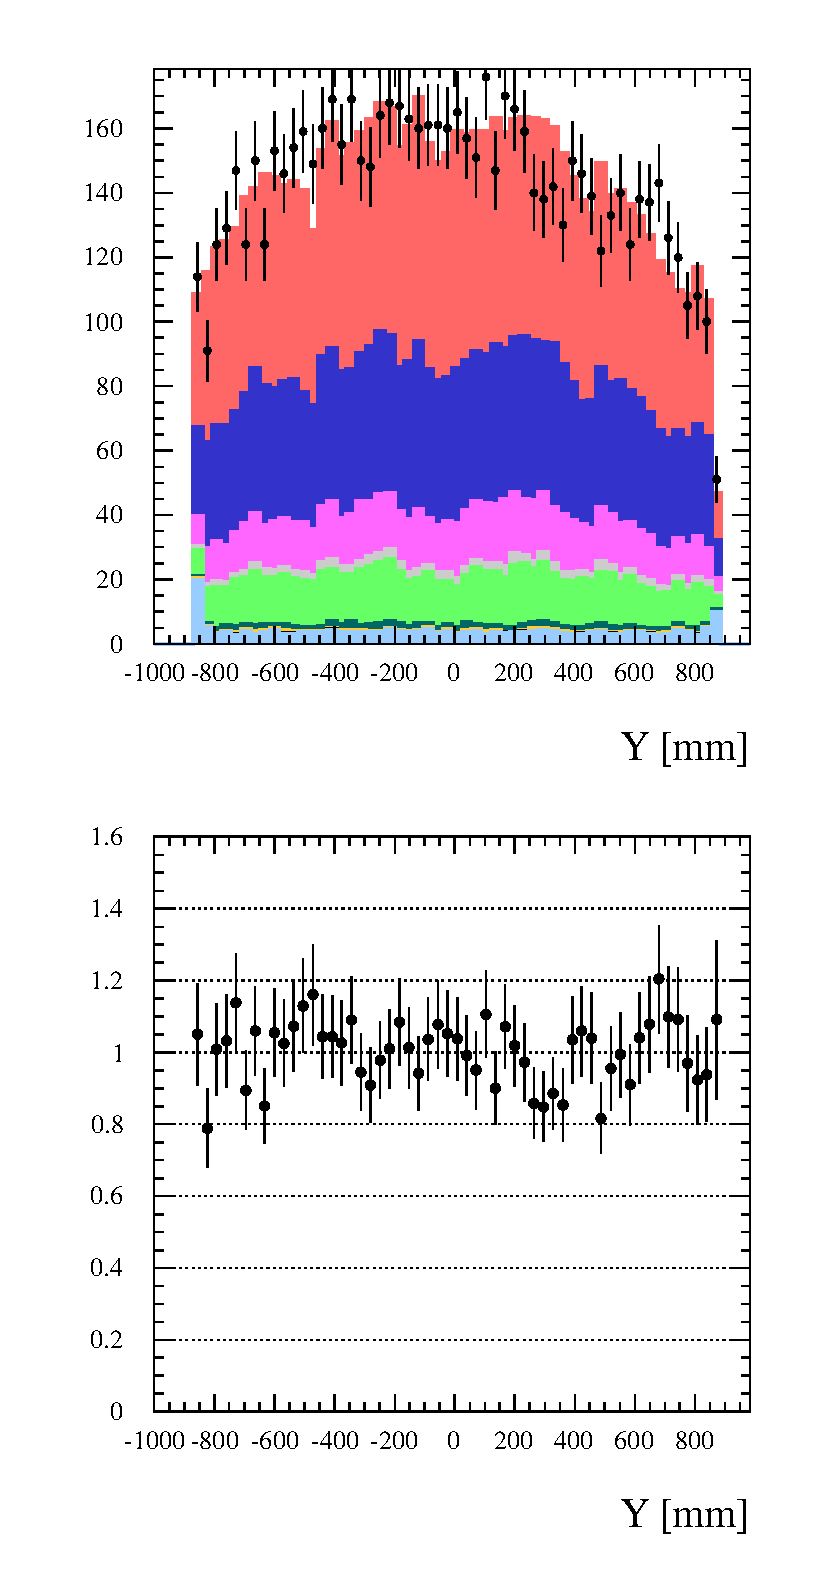
\includegraphics[width=3in]{Figures/P0DTrkYRun1Run2-normByRatio.eps}
  \caption{The candidate muon track start X and Y distributions 
Data to MC plots normalized by area.} 
  \label{fig:ResultsNormXY}%FIXME
\end{figure}

\begin{figure}[h]
  \centering
  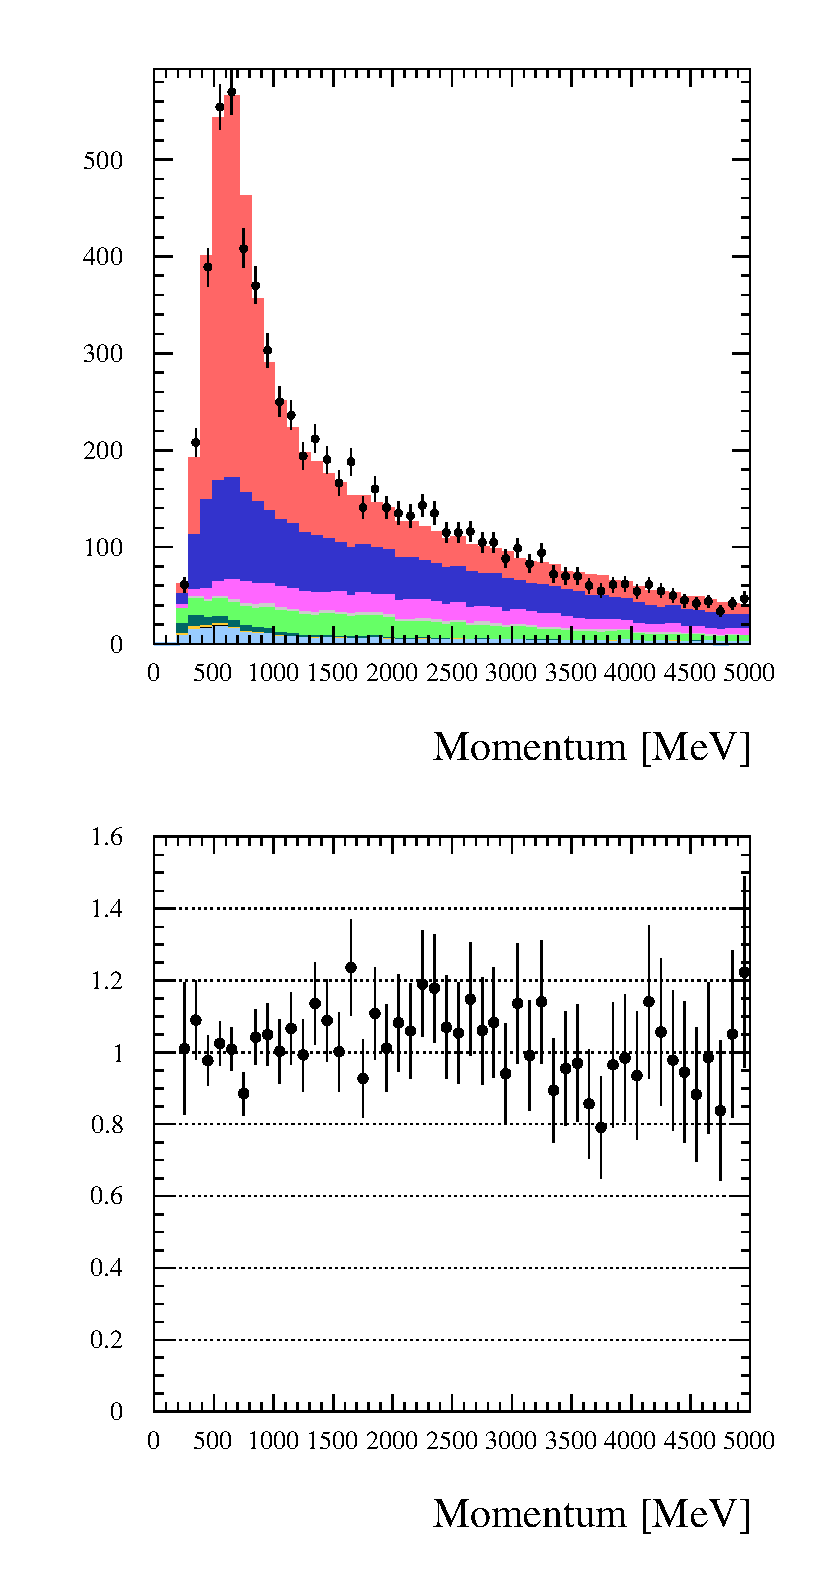
\includegraphics[width=3in]{Figures/P0DTrackerMomRun1Run2-normByRatio.eps}
  \includegraphics[width=3in]{Figures/P0DTrkZRun1Run2-normByRatio.eps}
  \caption{The candidate muon track Momentum and start Z distributions 
Data to MC plots normalized by area.}
  \label{fig:ResultsNormMomZ}%FIXME
\end{figure}

\begin{figure}[h]
  \centering
  \includegraphics[width=3in]{Figures/P0DTrkThetaRun1Run2-normByRatio.eps}
  \includegraphics[width=3in]{Figures/P0DTrkPhiRun1Run2-normByRatio.eps}
  \caption{The candidate muon track start $\theta$ and $\phi$ distributions 
Data to MC plots normalized by area.} 
  \label{fig:ResultsNormThetaPhi}%FIXME
\end{figure}

\clearpage

\subsection{\p0d Electronics Structure}
\label{sec:Appendix_p0delec}

The \p0d electronics is designed to have a live time and dead time structure that replicates the fine timing structure of the neutrino beam. The \p0d cycles through 23 `charge integration windows' or periods of live time per beam spill, where 8 of the windows capture the 8 beam bunches. These integration windows are 480ns long and are interleaved with 100ns of dead time. When a beam trigger is issued, the \p0d begins the cycle of 23 integration windows, and in this way is always able to keep the beam bunches beautifully centered within its live times. However, this is not the case for all types of cosmic events. 

FGD cosmics are triggered via coincident activity in FGD1 and FGD2. In addition, FGD timing is asynchronous to \p0d timing, so the \p0d is unable to always center an FGD cosmic track within a particular integration window. This leads to some number of cosmics tracks occuring right at the edge of a \p0d integration window and causing `fringe effects'. When the \p0d finds a hit near the edge of an integration window, by design it does not reconstruct the time. How close a hit can be to the edge of an integration window before it loses timing information is a function of Run number as well as whether we are using MC or Data. Values vary from 7.5ns from the edge in Run 1 Data to up to 70ns in MC. Large discrepancies such as this neccessitated cut 6 in Section \ref{sec:CosmicsEfficiency}. By requiring that the found hits are $>80$ns from the integration window edge, we negate any kind of fringe effects. This way we do not accidentally add a cosmics-only systematic effect to a study of beam events such as the inclusive analysis. 

\subsection{\p0d Matching Ambiguity}
\label{sec:Appendix_ambig}

A small percentage of the time, when a multi-track event is reconstructed in the \p0d with tracks entering TPC1, the matching algorithm fails to properly pair tracks together. This is an artifact of how \p0d reconstruction determines hit positions in a track. The \p0d extracts the X and Y positions of a hit from the scintillator bars ligned up along the X-axis and Y-axis respectively. However, When two tracks pass through the \p0d simultaneously, there are two X bars in each layer with energy deposited within. This yields two X positions for hits, namely $X_1$ and $X_2$. Similarly, in the Y-layers, we have two Y positions  $Y_1$ and $Y_2$. So \p0d reconstruction actually has two available combinations of X and Y positions for each 3D hit, i.e. ($X_1$, $Y_1$) and ($X_2$, $Y_2$) or ($X_1$, $Y_2$) and ($X_2$, $Y_1$). Depending on whether the correct combination is chosen, the algorithm can provide a set of reconstructed tracks that is a mirror image of the proper result. If the mirror image is chosen, then when the matching algorithm attempts to pair together \p0d and Tracker tracks, while it may succeed in one projection, it will always fail in the other. As this effect is essentially a combinatorial artifact, we observe the `ambiguous' track reconstruction failure mode in both Data and MC. A possible solution is to use TPC1 tracks as seeds to select the correct combination of X and Y positions, but this algorithm does not exist in the Production 4 suite of software pacakages.

\subsection{Sand Muon Matching Efficiency Cross Check}
\label{sec:Appendix_sandmuoneff}

In Production 4, Sand Muons were used as one of two independent samples 
to investigate and cross-check the reconstruction and matching efficiencies of the analysis. 
As previously mentioned, sand muons have a similar bunched timing structure 
to events from the beam which makes them an excellent unbiased sample 
to cross check the efficiency systematic. 
The matching efficiency has been outlined above.\\

The pre-selection, i.e. the denominator cuts, 
are exactly the same as the FGD cosmics sample 
except for step 6. 
For the sand muon sample, it is not necessary to have 
a 'good hit' finding algorithm like the FGD cosmics sample. 
Again, please refer to the appendix for greater detail. 
The matching cuts also exactly mimic the FGD cosmics section.\\

Figures \ref{fig:dRetcSM} and \ref{fig:dS_dT} show 
the same matching parameters as the cosmics sample 
but evaluated for the sand muon case. 
{\color{red}
In Fig. \ref{fig:dS_dT} one does notice that the MC $\Delta$T 
distribution 
%in the can of the snad muon sample 
has entries were the time difference are around zero, 
whereas the FGD cosmic MC distribution (Fig. \ref{fig:eff_dSdT})
has all the time difference shifted from zero. 
The reason for this 
%difference comes from  
lays in the fact that the 
Tracker track uses FGD or \p0d for its time reference.
While the sand muon sample has a small fraction of 
events where the Tracker track utilizes the \p0d as the time reference, 
the FGD cosmics sample uses, by design, only the FGD as 
its time reference.\\
}

Figure \ref{fig:eff(p)_eff(theta)} then shows 
the data and MC efficiencies with error 
and have been evaluated in the same manner 
as Section \ref{sec:CosmicsEfficiency}. 
The efficiencies from the sand muon sample 
are $98.22\%\pm 0.19\%$ for Data and $98.31\%\pm 0.18\%$ for MC.

%figure 1: dr, dx, dy
\begin{figure}
\centering
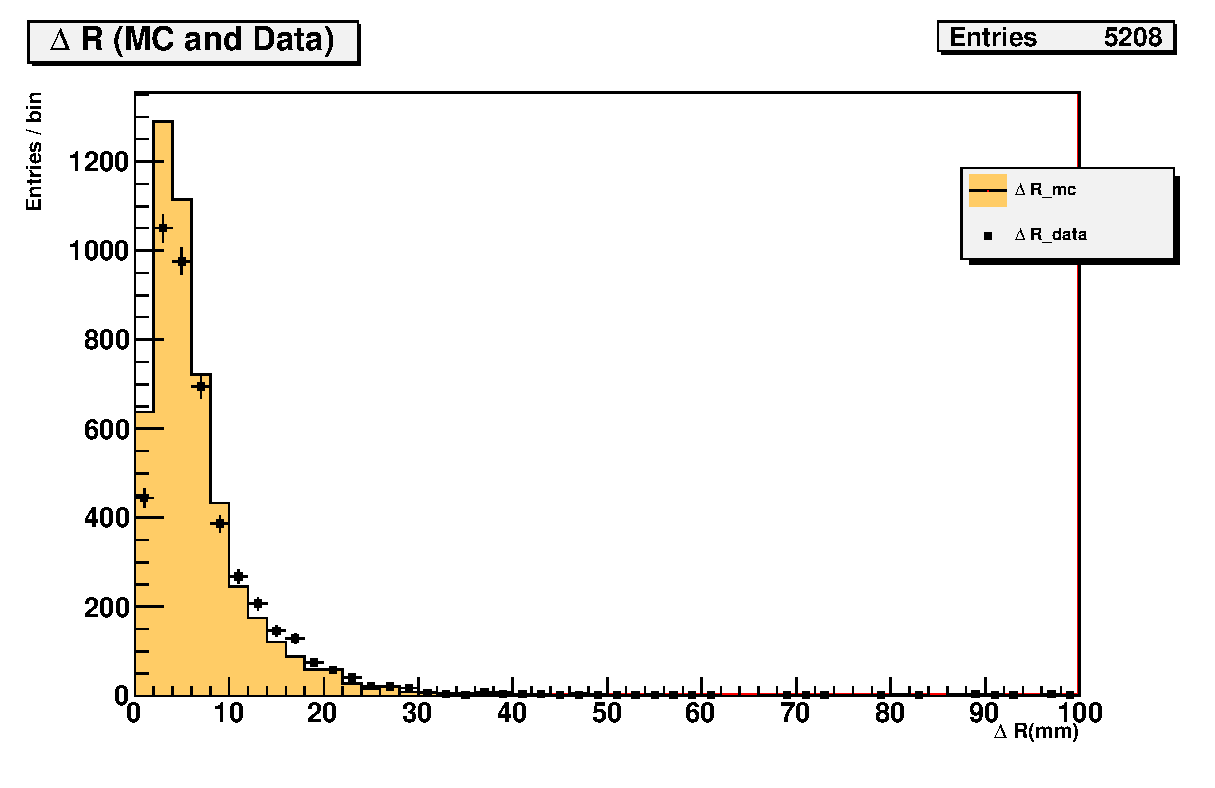
\includegraphics[width=2in]{Figures/Systematics/SandMuonEfficiencyPlots/C_34.eps}
\includegraphics[width=2in]{Figures/Systematics/SandMuonEfficiencyPlots/C_35.eps}
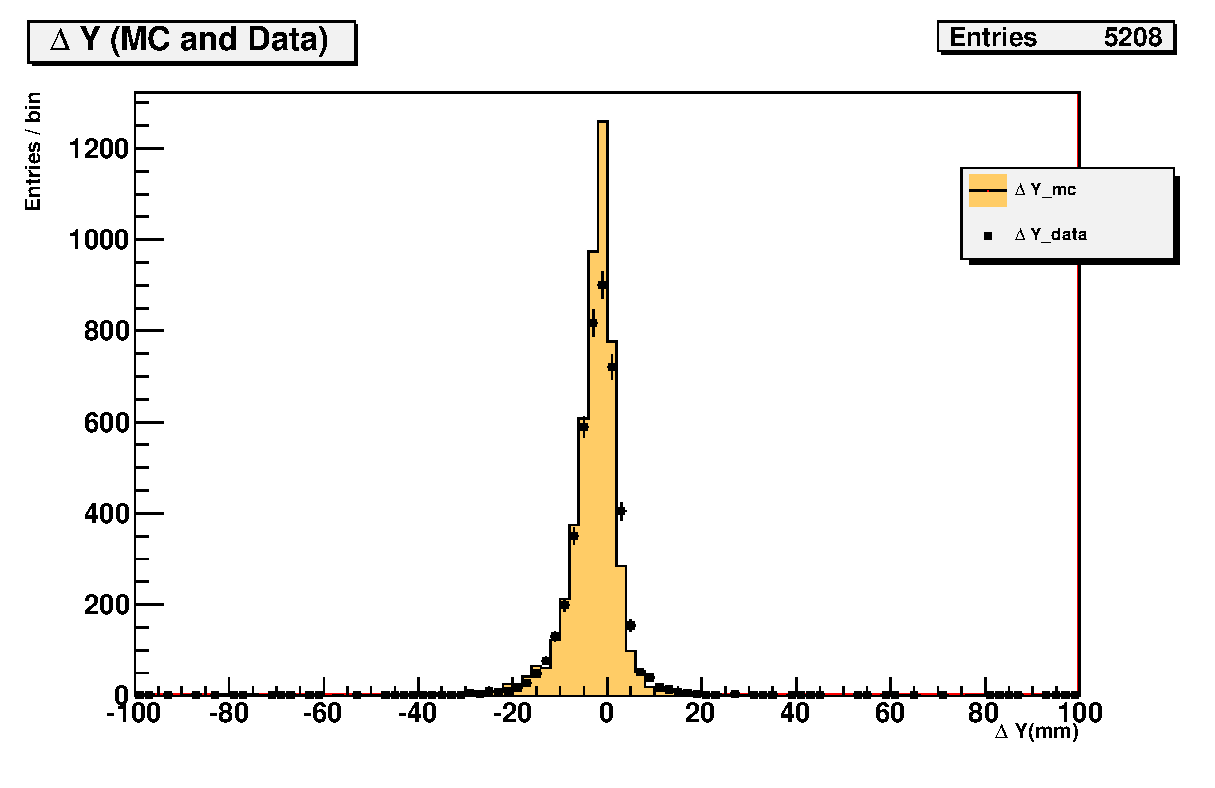
\includegraphics[width=2in]{Figures/Systematics/SandMuonEfficiencyPlots/C_36.eps}
\caption{Matching Parameters $\Delta$ R, $\Delta$ X, and $\Delta$ Y 
for sand muons. 
The matching cut is applied only on $\Delta$ R. 
Black dots with error bars denote data while the orange fill is monte carlo.}
\label{fig:dRetcSM}
\end{figure}


%figure 2 dt, sin(dtheta)
\begin{figure}
\centering
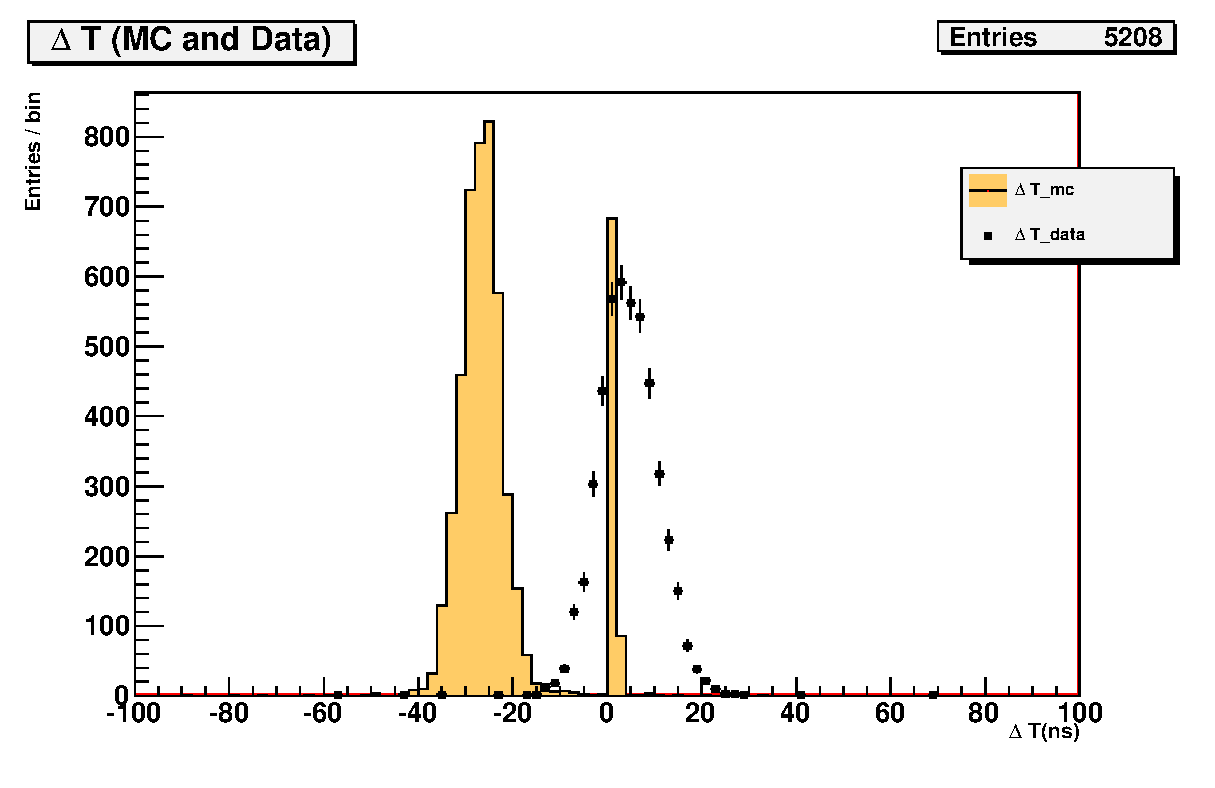
\includegraphics[width=2.5in]{Figures/Systematics/SandMuonEfficiencyPlots/C_37.eps}
\includegraphics[width=2.5in]{Figures/Systematics/SandMuonEfficiencyPlots/C_42.eps}
\caption{Sand muons matching parameters \(\sin \theta\) and \(\Delta T\). 
The difference in \(\Delta T\) is due to the the decision of 
the Tracker track to use the FGD or \p0d as its time reference.} 
\label{fig:dS_dT}
\end{figure}

%figure 3 Eff(P), Eff(theta)
\begin{figure}
\centering
\includegraphics[width=3in]{Figures/Systematics/SandMuonEfficiencyPlots/C_52.eps}
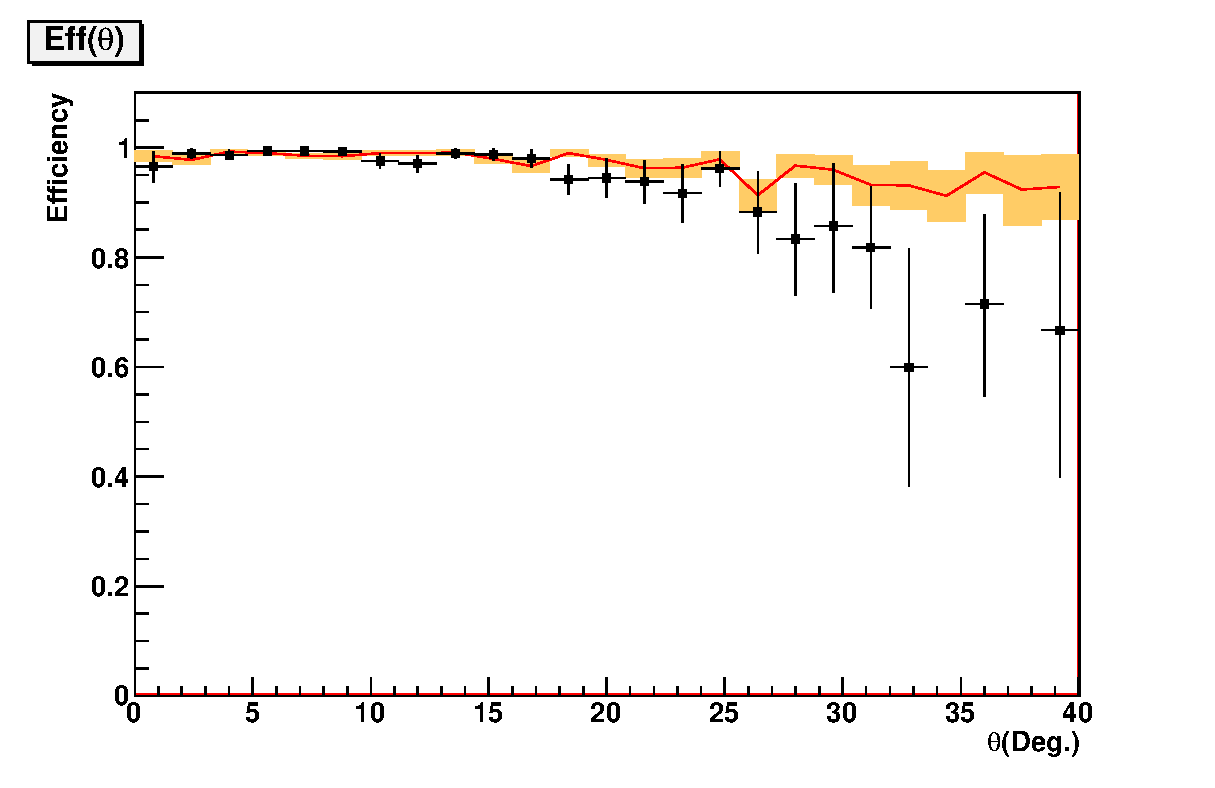
\includegraphics[width=3in]{Figures/Systematics/SandMuonEfficiencyPlots/C_51.eps}
\caption{\label{fig:eff(p)_eff(theta)}Sandmuon efficiencies as a function of Momentum and \(\theta\). Black dots are data and red line is the MC. The orange fill shows the error on the MC. We note that the data and MC efficiencies tracks each other as a function of both kinematic variables.}
\end{figure}


\subsection{\p0d and TPC Alignment}
\label{sec:Appendix_align}

Using the FGD Cosmics sample as well as the Sand Muon selection, we have found strong evidence that there is a difference between the `as-built' detector alignment and the input geometry used for reconstruction. Specifically, the geometry has a gap between the \p0d and TPC that is 10mm to 12mm larger than the `as-built' configuration. This effect can be seen in a correlation between the matching parameter residuals ($\Delta Y$ and $\Delta X$) and the steepness of the matched track. For an explanation of the matching residuals, please see the Section describing our reconstruction procedure. 

\begin{figure}
  \centering
  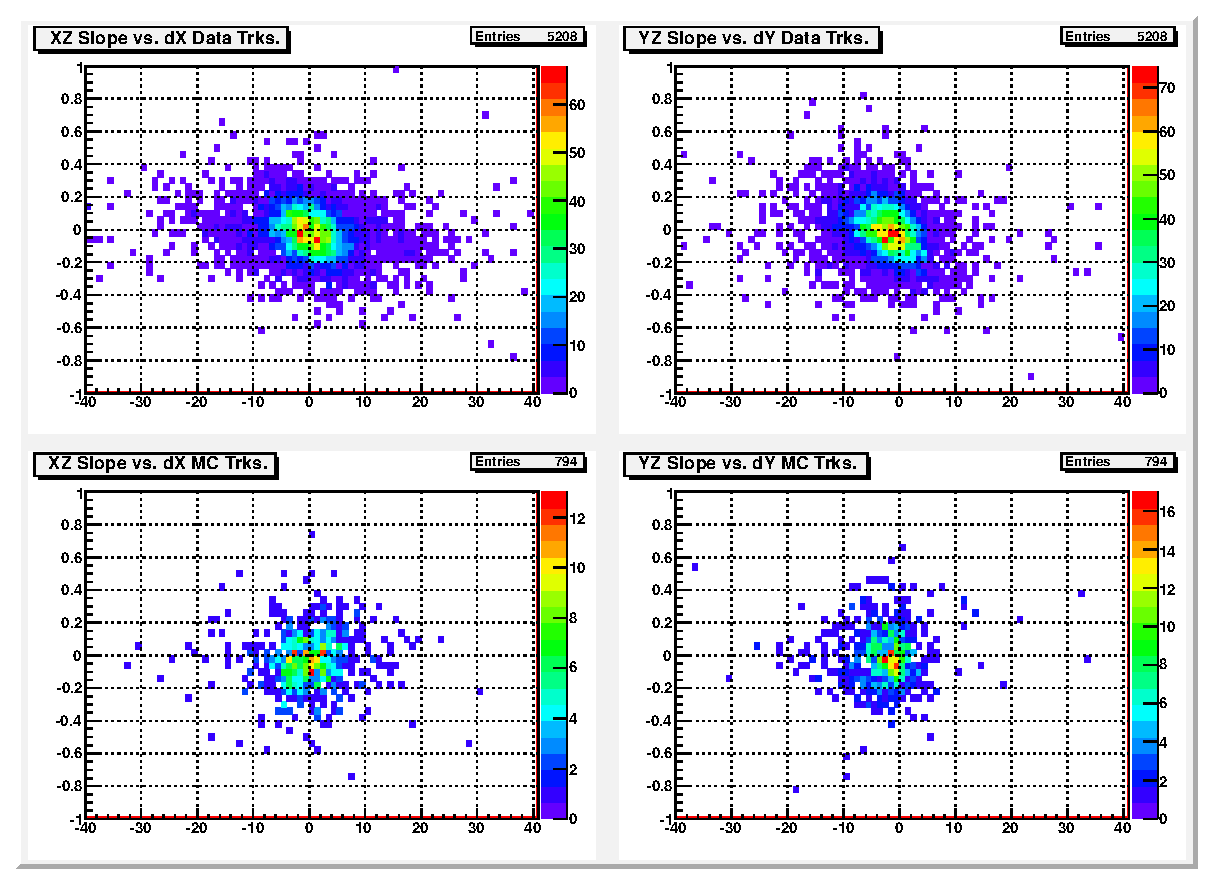
\includegraphics[width=6in]{Figures/Appendix/cdy_SM.eps}
  \caption{Top Left: XZ linear slope of track vs. $\Delta X$ residual for sand muons in Data. Top Right: YZ linear slope of track vs. $\Delta Y$ residual for sand muons in Data. Bottom Left: XZ linear slope of track vs. $\Delta X$ residual for sand muons in MC. Bottom Right: YZ linear slope of track vs. $\Delta Y$ residual for sand muons in MC.} 
  \label{fig:cdy_SM}%FIXME
\end{figure}

\begin{figure}
  \centering
  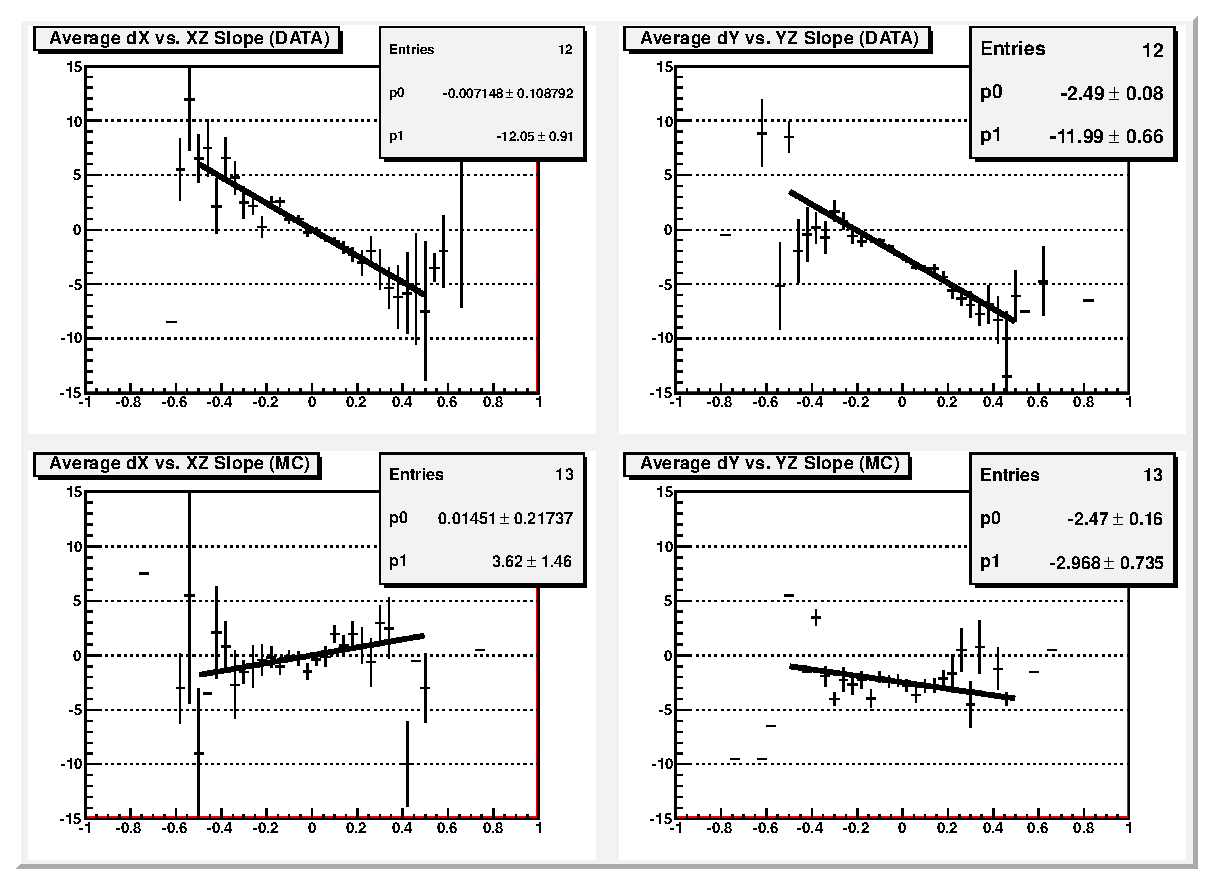
\includegraphics[width=6in]{Figures/Appendix/cprof_SM.eps}
  \caption{Top Left: Average $\Delta X$ residual vs. XZ linear slope of track for sand muons in Data. Top Right: Average $\Delta Y$ residual vs. YZ linear slope of track for sand muons in Data. Bottom Left: Average $\Delta X$ residual vs. XZ linear slope of track for sand muons in MC. Bottom Right: Average $\Delta Y$ residual vs. YZ linear slope of track for sand muons in MC.} 
  \label{fig:cprof_SM}%FIXME
\end{figure}

\begin{figure}
  \centering
  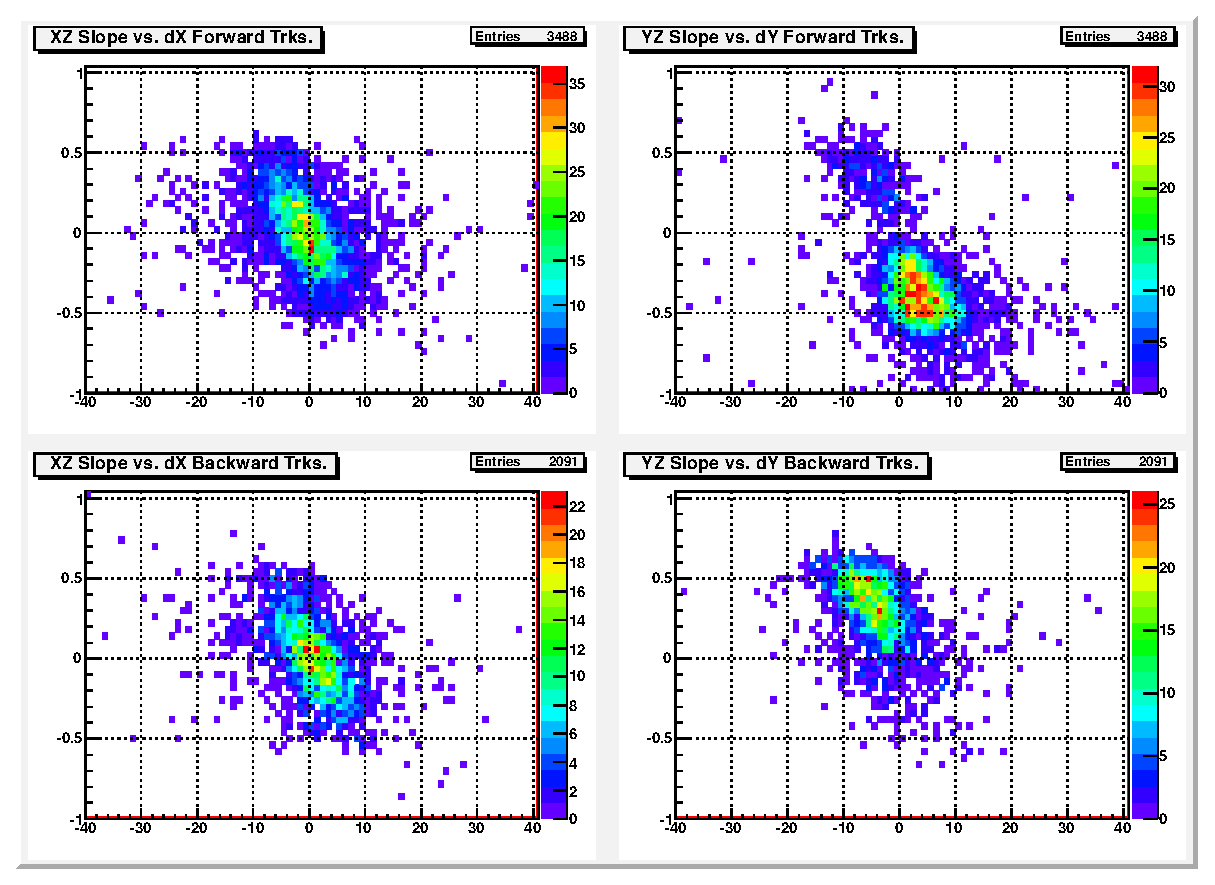
\includegraphics[width=6in]{Figures/Appendix/cdy_data.eps}
  \caption{Plots for Cosmics Data. Top Left: XZ linear slope of track vs. $\Delta X$ residual. Top Right: YZ linear slope of track vs. $\Delta Y$ residual. Bottom Left: XZ linear slope of track vs. $\Delta X$ residual. Bottom Right: YZ linear slope of track vs. $\Delta Y$ residual.} 
  \label{fig:cdy_data}%FIXME
\end{figure}

\begin{figure}
  \centering
  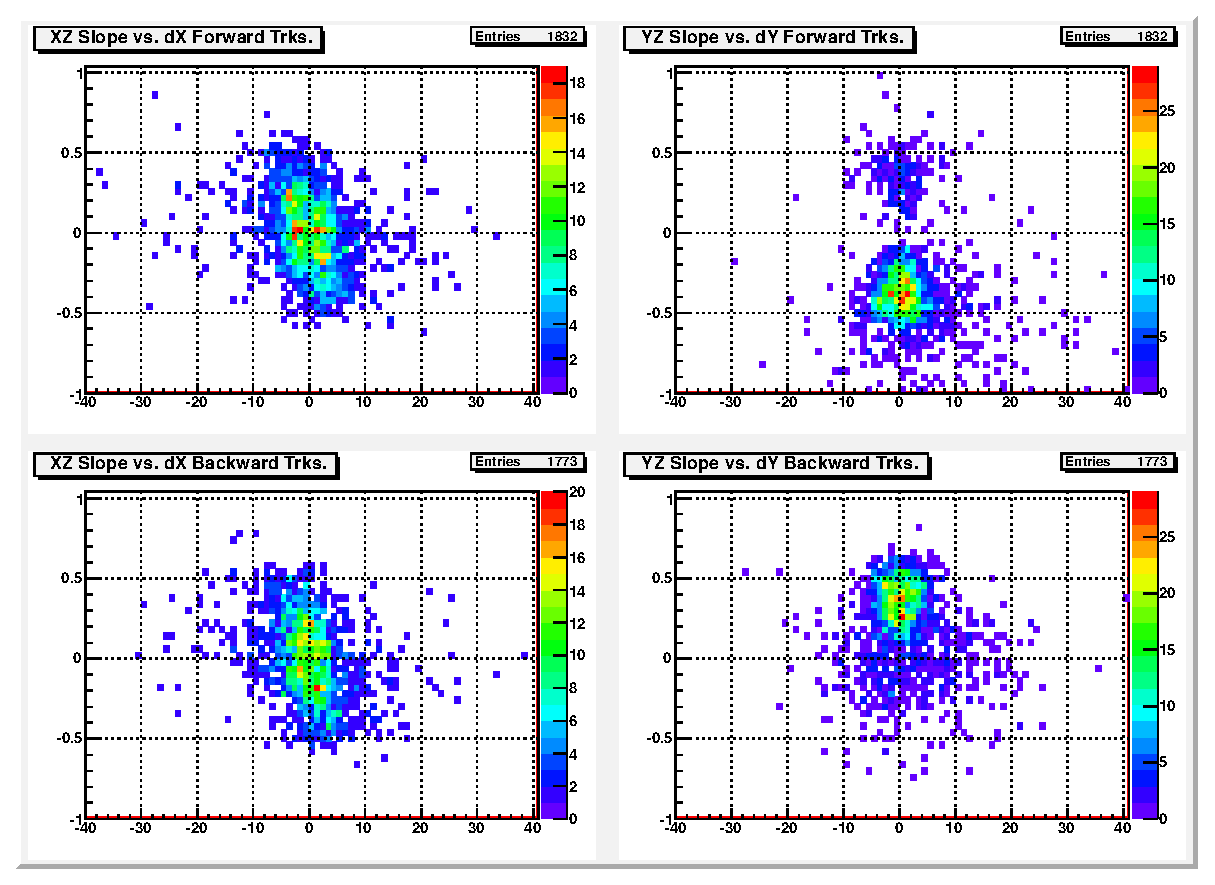
\includegraphics[width=6in]{Figures/Appendix/cdy_mc.eps}
  \caption{Plots for Cosmics MC. Top Left: XZ linear slope of track vs. $\Delta X$ residual. Top Right: YZ linear slope of track vs. $\Delta Y$ residual. Bottom Left: XZ linear slope of track vs. $\Delta X$ residual. Bottom Right: YZ linear slope of track vs. $\Delta Y$ residual.} 
  \label{fig:cdy_mc}%FIXME
\end{figure}

\begin{figure}
  \centering
  \includegraphics[width=6in]{Figures/Appendix/cprof_data.eps}
  \caption{Plots for Cosmics Data. Top Left: Average $\Delta X$ residual vs. XZ linear slope of track. Top Right: Average $\Delta Y$ residual vs. YZ linear slope of track. Bottom Left: Average $\Delta X$ residual vs. XZ linear slope of track. Bottom Right: Average $\Delta Y$ residual vs. YZ linear slope of track.} 
  \label{fig:cprof_data}%FIXME
\end{figure}

\begin{figure}
  \centering
  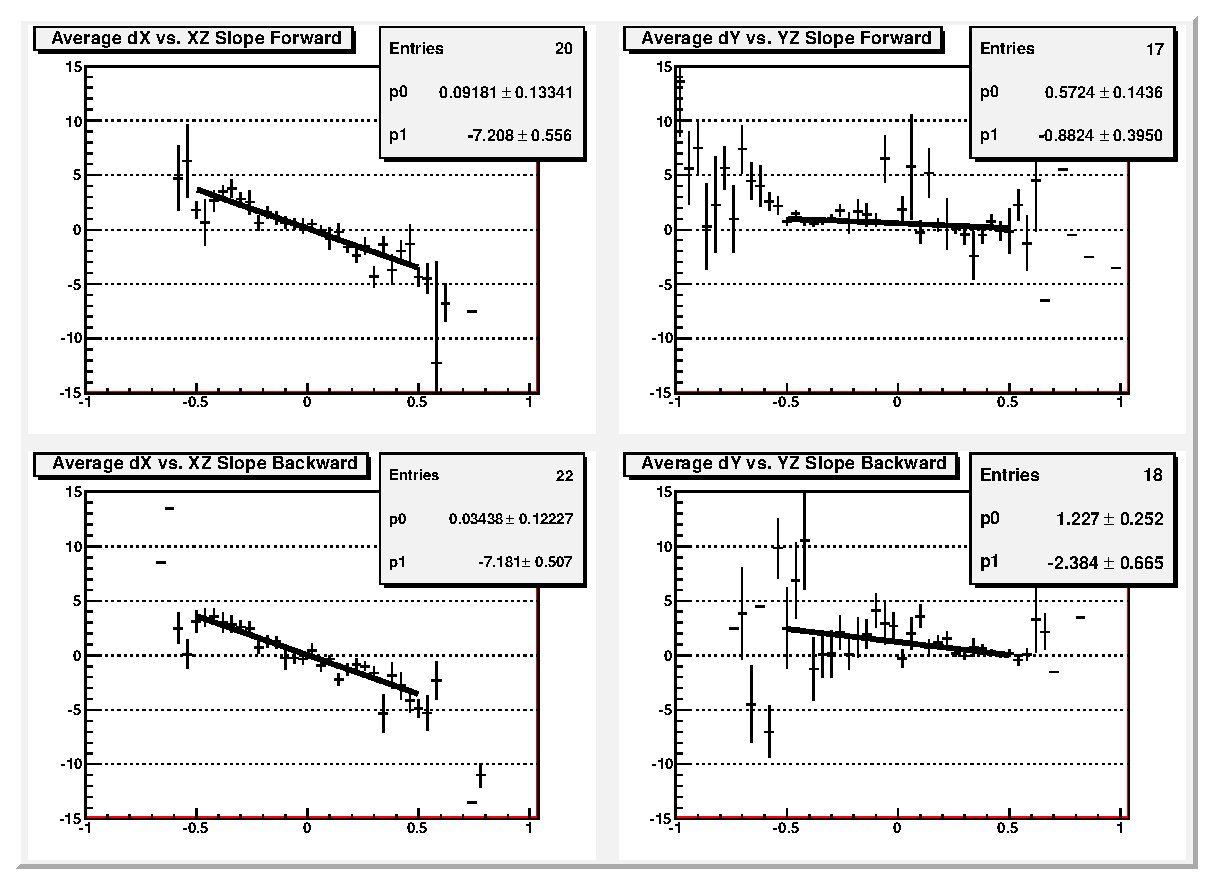
\includegraphics[width=6in]{Figures/Appendix/cprof_mc.eps}
  \caption{Plots for Cosmics MC. Top Left: Average $\Delta X$ residual vs. XZ linear slope of track. Top Right: Average $\Delta Y$ residual vs. YZ linear slope of track. Bottom Left: Average $\Delta X$ residual vs. XZ linear slope of track. Bottom Right: Average $\Delta Y$ residual vs. YZ linear slope of track.} 
  \label{fig:cprof_mc}%FIXME
\end{figure}



To measure the correlation between residuals and steepness, we first calculate the linear slope of each matched track in the XZ and YZ projections. The slope is approximated by drawing a line from the start of the track to the point where the track exits the \p0d. For the purposes of this exercise, the small expected curvature of the track is ignored. These linear slopes are plotted against the residuals in the XZ and YZ projections and the results are shown in Figures \ref{fig:cdy_SM} (sand muons) and \ref{fig:cprof_SM} (cosmics). A profile of these scatter plots then yields the Average residual vs. linear slope of the track. A quick linear fit to the profile plots allows us to extract the difference between the geometry and `as-built' versions of the detectors. For example, a fit slope of 10mm means that for a track of slope 1 (i.e. 45 degrees) we have a shift in the residual of 10mm. Since this is a 45 degree track, this also implies that the Z axis misalignment is also 10mm. The profile plots for sand muons and cosmics for both data and MC are shown in Figures \ref{fig:cprof_SM}, \ref{fig:cprof_data} and \ref{fig:cprof_mc}.

To conclude, we note that both sand muons and cosmics suggest that there is a 10mm to 12mm difference between the geometry used for reconstruction and the `as built' detector. The fit slope of the sand muon MC sample is consistent with a horizontal line, and shows no correlation between residuals and track steepness. We do note some tension in the XZ projection of the cosmics MC with the rest of our plots as there is a small correlation between the $\Delta X$ residual and track steepness. This is unexpected as we would not normally expect the reconstruction geometry to differ from the geometry used to generate events. However, upon further investigation, we found that the geometries for Production 4 have been changed several times and may be consistent with our findings. Regardless, we reiterate that the matching efficiency systematic is designed to quantify and find these exact problems. The values we have evaluated in the systematics chapter conservatively account for these alignment differences by allowing for the largest possible alignment error (see the sand muon sample and summary of the matching efficiency systematic section). 
